\documentclass{llncs}
\usepackage[utf8]{inputenc}
\usepackage[spanish]{babel}
\usepackage{graphicx}
\usepackage{listings}
\usepackage{xcolor}
\usepackage{amsmath}
\usepackage{hyperref}

\hypersetup{
    colorlinks=true,
    urlcolor=blue
}

\lstset{
    basicstyle=\ttfamily\footnotesize,
    breaklines=true,
    frame=single,
    numbers=left,
    keywordstyle=\color{blue},
    commentstyle=\color{gray},
}

% Configuración de encabezados y pies de página
\pagestyle{headings}
\title{Proyecto Final de Compilación: Diseño e Implementación de un Compilador para el Lenguaje HULK}
\author{Claudia Hernández Pérez \and Joel Aparicio Tamayo \and Kendry J. Del Pino Barbosa}
\institute{Facultad de Matemática y Computación, Universidad de La Habana} 

\begin{document}

\maketitle

\begin{abstract}
Este documento describe el diseño e implementación de un compilador para HULK en el lenguaje C. El 
diseño del compilador agrupa 4 partes: \textit{lexer}, \textit{parser}, \textit{chequeo semántico} y \textit{generación de código}.

El \textit{lexer} y el \textit{parser} se basan en los frameworks proporcionados por Lex y Yacc, respectivamente, aunque el proyecto cuenta con
una implementación propia de un \textit{lexer} basado en la teoría de autómatas finitos. El \textit{chequeo semántico} es responsable de validar las reglas del lenguaje,
reduciendo los errores en tiempo de ejecución. Para ello se ha implementado el patrón Visitor, que permite recorrer el árbol de sintaxis abstracta (AST) y aplicar las reglas semánticas correspondientes. Además,
cuenta con una arquitectura que permite la unificación de expresiones con tipos, lo que facilita la inferencia. Finalmente, la \textit{generación de código} se realiza mediante un generador de código intermedio que
también implementa el patrón Visitor para traducir el AST a código LLVM.

Al ejecutar el compilador de HULK, se genera un \texttt{output.ll} en la carpeta \textit{build}, donde se encuentra 
el código generado, y luego se invoca al compilador de LLVM para ejecutar dicho archivo, y devolver la salida del programa.
\vspace{10pt}
\keywords{Compilador \and Lexer \and Parser \and Chequeo Semántico \and AST \and Scope \and Generación de código \and LLVM \and Inferencia \and Expresión \and Tipo}
\end{abstract}

\section{Introducción}
Los compiladores son herramientas fundamentales en la ciencia computacional, actuando como puentes entre abstracciones de alto nivel y ejecución eficiente. Específicamente, HULK (Havana University Language for Kompilers),
es un lenguaje de programación didáctico, seguro de tipos, orientado a objetos e incremental. Este proyecto tiene la finalidad de compilar un subconjunto de dicho 
lenguaje, siendo consistente con las especificaciones en su \href{https://matcom.in/hulk/guide/intro}{definición formal}, aunque añadiendo algunas extensiones sintácticas propias.

Para compilar HULK, se ha diseñado un flujo de trabajo sencillo y por capas. El punto de entrada del programa es 
el archivo \texttt{main.c}, que intenta leer un archivo \texttt{script.hulk} en formato de cadena de texto y luego invoca al \textit{lexer} y al \textit{parser} para generar un árbol de sintaxis abstracta (AST). Posteriormente,
si no hubo errores léxicos ni sintácticos, se realiza el \textit{chequeo semántico} a partir del nodo raíz del AST. Finalmente, si no hubo errores semánticos, se procede a la \textit{generación de código} intermedio, que se traduce a código LLVM. En
este punto concluye el proceso de compilación, generando un archivo \texttt{output.ll} en la carpeta \textit{build}. Para cada proceso del programa (compilación, ejecución, limpieza) existe una receta en el \texttt{Makefile} que lo ejecuta: 
\begin{lstlisting}[language=bash]
make compile // para compilar y generar el build/outout.ll
make execute // para ejecutar el compilador de LLVM 
make clean // para limpiar el directorio de compilacion
\end{lstlisting}

A continuacón se detallan los disitntos aspectos de la implementación.
\vspace{10pt}
\section{Lexer y parser}


\begin{figure}[h]
\centering
% \includegraphics[width=0.8\textwidth]{compiler_phases.pdf}
\caption{Arquitectura modular del compilador}
\label{fig:arquitectura}
\end{figure}

\vspace{10pt}
\section{Análisis semántico}

Como se ha mencionado anteriormente, la entrada del \textit{chequeo semántico} es el nodo raíz del AST, que es donde comienzan los chequeos, utilizando el
patrón Visitor. La implementación de este patrón (ver Figura~\ref{fig:visitor}) contiene: 
\begin{itemize}
    \item \textbf{Funciones de visita para cada tipo de nodo del AST}: Para cada nodo hay una función que sabe analizarlo y aplicar las reglas semánticas correspondientes.
    \item \textbf{Lista de errores semánticos encontrados}: Se mantiene una lista de errores semánticos encontrados durante el análisis, que se reportan al usuario al finalizar el chequeo.
    \item \textbf{Cantidad de errores semánticos encontrados}: Longitud de la lista de errores encontrados (recordar que en C no se puede obtener el tamaño de un array dinámico, por lo que se debe mantener un contador)
    \item \textbf{Recolector de contextos}: Se encarga de recolectar todas las declaraciones de funciones y tipos en el contexto actual, antes de analizarlas
    \item \textbf{Nombre de la función actual}: Se mantiene el nombre de la función que se está analizando actualmente, para evitar tener que subir de nuevo en el AST cuando se necesite, como por ejemplo al usar: \textit{base(...)}
    \item \textbf{Tipo actual}: Similar al caso anterior e igualmente necesario para el ejemplo brindado, pues en el caso del uso de \textit{base(...)} se debe saber el tipo de la clase actual para poder buscar el método en algún ancestro.
\end{itemize}

\begin{figure}[h]
\centering
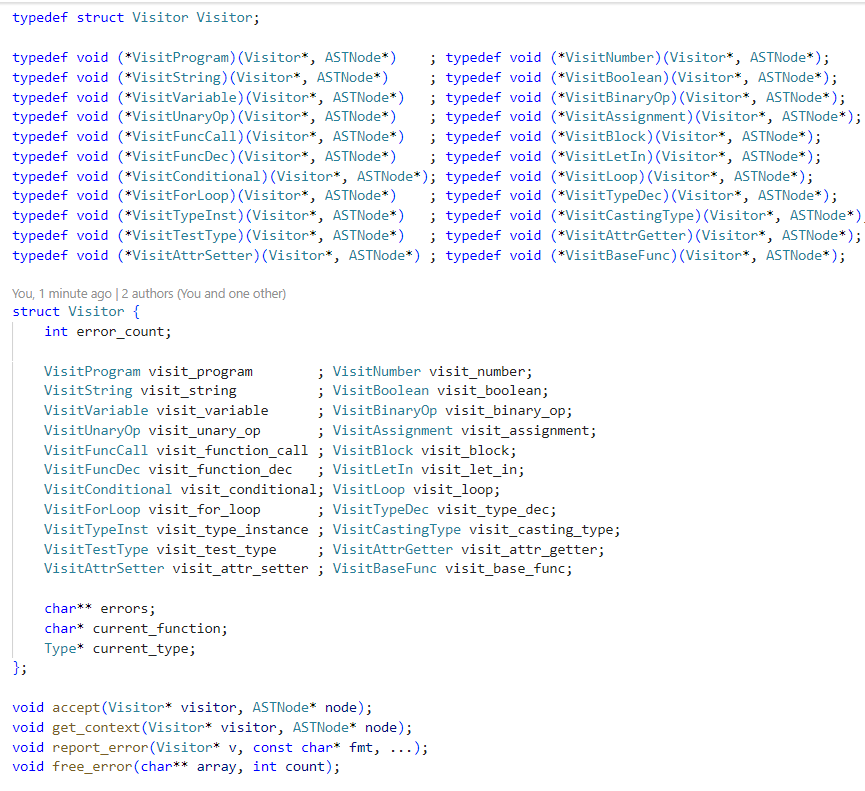
\includegraphics[width=1\textwidth]{images/visitor.png}
\caption{Implementación del patrón Visitor para el chequeo semántico}
\label{fig:visitor}
\end{figure}

El inicio del análisis se encuentra en el archivo \texttt{semantic.c}, donde primero se inicializa el visitor y luego se visita al nodo raíz del AST. La implementación de la función de
visita de ese nodo, primero realiza las declaraciones de tipos y funciones builtin del lenguaje, luego recoge el contexto del programa y finalmente visita cada uno de sus
descendientes. Al concluir el análisis, se imprimen en consola (con fuente en color Rojo) los errores reportados, y continúa el flujo del compilador. 
Para el chequeo semántico, cada nodo contará con un tipo de retorno, un ámbito (scope) y un contexto asociados (cada campo cumple una función específica y serán analizados posteriormente), y en caso de no
especificar lo contrario, se asumirá de aquí en adelante que en cada visita el ámbito y contexto padres son los del nodo padre (NULL en caso de la raíz).

Ahora se explicará detalladamente cada uno de 
los chequeos que se realizan a cada nodo.

\subsection{Análisis de expresiones básicas}

En la implementación, se consideran como expresiones básicas a los literales (números, cadenas, booleanos), operaciones unarias (!, -), 
operaciones binarias $(+, -, *, /, \%, ^, \&, |, ==, !=, <, >, <=, >=, @, @@)$, así como los bloques de expresiones.
\begin{enumerate}
    \item \textbf{Literales}: En el caso de los números y booleanos, las funciones de visita están vacías, pues no hay nada que chequear; sin embargo,
    en el caso de las cadenas, se verifica que los caracteres de escape utilizados (si los hay) sean correctos.
    \item \textbf{Operaciones unarias}: Primero se visita al nodo de la expresión hija y luego se chequea la compatibilidad del tipo de dicha expresión con
    la operación unaria dada. (La compatibilidad de tipos con operadores se explicará más adelante). Luego se actualiza el tipo de retorno del nodo según el operador.
    \item \textbf{Operaciones binarias}: Similiar a las operaciones unarias, se visitan primeros los nodos de las expresiones con las que se quiere operar y luego 
    se chequea la compatibilidad de ambos tipos con el operador binario dado (La compatibilidad de tipos con operadores se explicará más adelante). Luego se actualiza el tipo 
    de retorno del nodo según el operador.
    \item \textbf{Bloques de expresiones}: Similar al nodo raíz, el nodo bloque funciona como un mini programa, por lo cual se recolecta primero su contexto y luego se visita cada uno de sus 
    descendientes, manteniendo siempre el último visitado para poder al final actualizar el tipo de retorno del nodo bloque con el tipo de su último descendiente. Si el bloque esta vacío, automáticamente 
    se le otorga tipo de retorno \texttt{Void}.
\end{enumerate}

\textbf{Compatibilidad de tipos con operadores}: En el archivo \texttt{type.c} se definen todas las reglas de compatibilidad de tipos. En el arreglo \texttt{operator\_rules} (ver Figura~\ref{fig:operadores}) se almacenan las reglas para los 
operadores de la forma \{\texttt{tipo de la izquierda, tipo de la derecha, tipo de retorno, operador}\}. En caso que un operador pueda utilizarse con varios tipos, como es el caso del '==' por ejemplo, aparece una regla por cada
uso del operador. De esta forma, es más sencillo revisar la compatibilidad de tipos con operadores, pues solo se tienen que recorrer las reglas y comparar los tipos izquierdos y derechos (NULL para los unarios) según el operador.

\begin{figure}
\centering
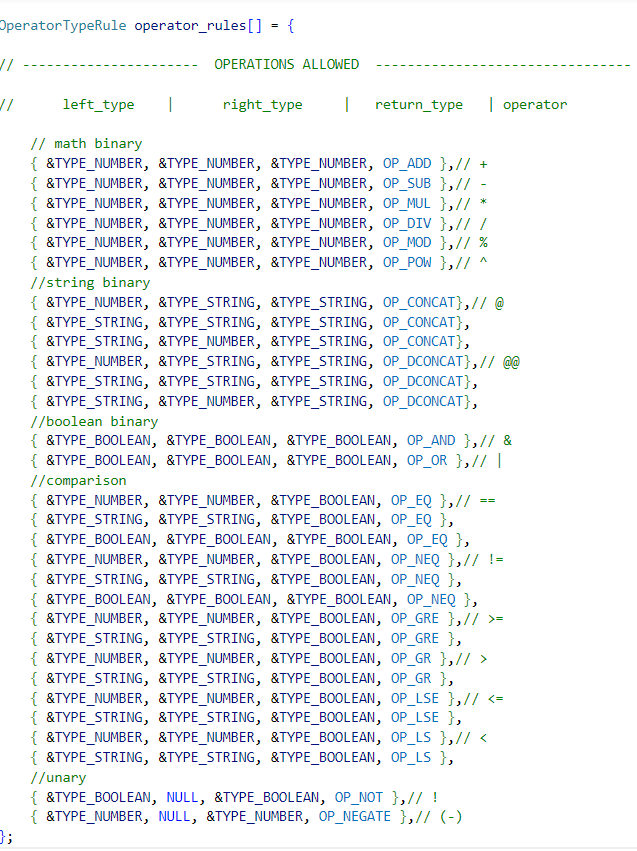
\includegraphics[width=1\textwidth]{images/op_rules.png}
\caption{Reglas para los operadores}
\label{fig:operadores}
\end{figure}

\textbf{Errores}: De manera general y como se expuso con anterioridad, en las expresiones básicas los errores más comunes son 
los respectivos a secuencias de escapes inválidas en cadenas e incompatibilidad con los operadores (ver ejemplo Figura~\ref{fig:errores_1}).
\begin{figure}[h]
\centering
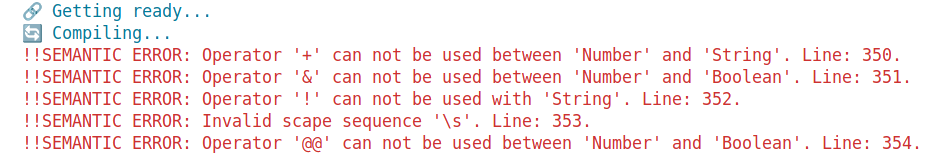
\includegraphics[width=1\textwidth]{images/basic_errors.png}
\caption{Errores comunes en expresiones básicas}
\label{fig:errores_1}
\end{figure}

\subsection{Análisis de variables y ámbitos (scopes)}

La revisión de variables, en general, contempla el chequeo de asignaciones, el uso de variables y
las expresiones \textit{let-in}. Para comprender mejor esta sección, se comenzará explicando la estructura 
de un \textit{scope} y las posibles acciones que se pueden realizar sobre él.

Un \textbf{scope}, en la implementación dada, es una estructura que contiene, a grandes rasgos, una tabla de
símbolos, una tabla de funciones y una tabla de tipos definidos, las cuales actúan como bases de datos para las
respectivas definciones en los distintos ámbitos del programa, además de una referencia al \textit{scope} padre.
Sobre los \textit{scopes} se pueden realizar diversas  acciones, iniciando claramente por su creación y
finalizando con su destrucción al concluir el chequeo semántico (en C la liberación de memoria es manual). Esas
acciones incluyen:
\begin{itemize}
    \item Guardar símbolos, funciones o tipos en las tablas.
    \item Buscar específicamente algún símbolo, función o tipo definidos.
    \item Inicializar tipos y funciones \textit{builtin}.
    \item Liberar memoria para cada tabla.
\end{itemize}

Luego de entender la estructura de los \textit{scopes}, se abordarán los distintos tipos de análisis realizados en el caso 
de las variables: 

\begin{enumerate}
    \item \textbf{Asignaciones}: La revisión comienza chequeando que el nombre dado a la variable no sea un \textit{keyword}, de lo contrario se reporta un error. También 
    con respecto a la variable, se verifica si fue tipada o no, y en caso que sí, se analiza que el tipo sea válido. Luego, se pasa al chequeo de la parte derecha de la asignación, 
    invocando su función de visita. Una vez termina de visitar la expresión de la derecha, se revisa la compatibilidad del tipo de dicha expresión con el tipo impuesto a la variable 
    (en caso de haber sido tipada, en otro caso no sucede nada) y se guarda en dependencia del operador de asignación. Si se utiliza \texttt{==} se crea un nuevo símbolo en el
    \textit{scope} padre, y en caso del operador destructivo \texttt{:=}, se busca el símbolo en la tabla de símbolos (de algún \textit{scope} ancestro) y se verifica que sean compatibles 
    los tipos de la inicialización y la reasignación. En caso que no, o que no se haya encontrado el símbolo se reportará error. En el caso del uso de asignación destructiva 
    el tipo de retorno del nodo es el mismo que el de la variable asignada (la cual toma el tipo de la expresión de la derecha si no fue tipada), y en caso contrario el retorno es \texttt{Void}.
    \item \textbf{Uso de variables}: Esta revisión es más sencilla, pues basta con buscar la variable en algún \textit{scope} ancestro y si no existe se reporta error.
    \item \textbf{Let-in}: Esta expresión esta compuesta por un conjunto de asignaciones y un cuerpo. Por tanto, la revisión consta de 
    visitar cada una de las asignaciones y luego visitar el cuerpo. El tipo de retorno es el mismo que el tipo de retorno del cuerpo.
\end{enumerate}

\textbf{Errores}: Como se expuso anteriormente, los errores detectados en estas revisiones son: tipo no definido al tipar una variable, 
incompatibilidad de tipos en asignaciones (en el caso de las que son tipadas), reasignar una variable que no ha sido inicializada antes, intentar reasignar una variable con un tipo incompatible 
con el tipo de su inicialización, variable indefinida, entre otros.  (ver ejemplo Figura~\ref{fig:errores_2}).
\begin{figure}[h]
\centering
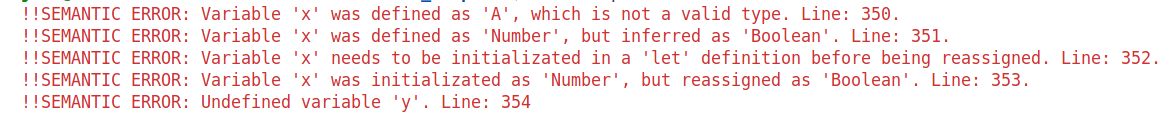
\includegraphics[width=1\textwidth]{images/var_errors.png}
\caption{Errores comunes en variables}
\label{fig:errores_2}
\end{figure}

\subsection{Análisis de funciones}

El análisis de funciones agrupa dos tipos de revisiones: chequeo de la declaración y chequeo del llamado. Como las funciones pueden declararse en cualquier sección del programa 
se necesita primero recoger el contexto de todas las declaraciones. Para eso se utiliza una estructura denominada \textit{context}.

El \textit{context}, al igual que el \textit{scope} sirve como una base de datos, pero dedicada a guardar los nodos de las declaraciones de funciones (o tipos, que se verán más adelante). 
Sobre un \textit{context} se puede: 
\begin{itemize}
    \item Guardar una declaración.
    \item Buscar una declaración.
\end{itemize}

Ahora se explicará cada una de las revisiones dichas anteriormente:
\begin{enumerate}
    \item \textbf{Llamado a funciones}: Lo primero que se se hace es visitar cada uno de los argumentos. Luego se busca la función en el \textit{context} y se revisa su declaración para que queden guardados sus 
    datos en el \textit{scope} (en caso de haber sido o estar en proceso de ser revisada, no sucede nada). Finalmente se chequea que la cantidad de argumentos y los tipos de los argumentos coincidan con la declaración 
    de dicha función y se actualiza el tipo de retorno del nodo del llamado con el guardado en el \textit{scope}.
    \item \textbf{Declaración de funciones}: Al igual que con la asignación de variables, se comienza revisando que el nombre de la función no sea una \textit{keyword}. Después se hace un pequeño chequeo para descartar que existan 
    nombres de parámetros repetidos. Luego se pasa a declarar en el \textit{scope} de la declaración cada uno de los parámetros para que sean accesibles en el cuerpo de la función, revisando primero que si son tipados, tengan un tipo válido. Al terminar 
    con los parámetros, se chequea el cuerpo, comenzando por ver si la función tiene un tipo de retorno definido, y en ese caso igualmente revisar que sea un tipo válido y más adelante que sea compatible con el tipo inferido del cuerpo; y luego se llama a su
    función de visita.
\end{enumerate}

\textbf{Errores}: Existen diversos tipos de errores que se detectan en estas revisiones: incompatibilidad de tipos en los parámetros, en el retorno, repetición de un 
mismo símbolo en los argumentos de una declaración, función no definida, cantidad de argumentos no compatible, entre otros (ver ejemplo Figura~\ref{fig:errores_3}).
\begin{figure}[h]
\centering
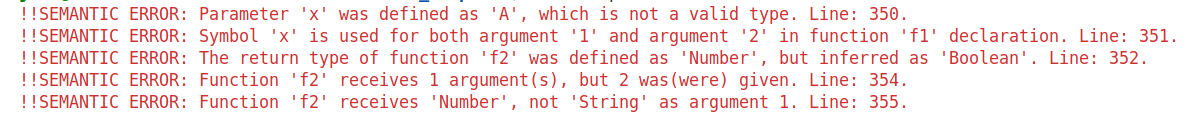
\includegraphics[width=1\textwidth]{images/func_errors.png}
\caption{Errores comunes en funciones}
\label{fig:errores_3}
\end{figure}

\subsection{Análisis de condicionales y ciclos}

La revisión de condicionales y ciclos se centra precisamente en revisar cada una de esas expresiones, además de un tipo 
especial de condicional: \textit{q-conditional}. A continuacón se explican cada una de ellas detalladamente: 
\begin{enumerate}
    \item \textbf{Condicionales}: Las condicionales tienen tres partes: condición, bloque para el \textit{if}, bloque para el \textit{else} 
    (el \textit{elif} es convertido automáticamente por el compilador a un \textit{else if}). La revisión ocurre secuencialmente por esas tres partes: 
    se visita el nodo de la condición y se verifica que su tipo de retorno sea booleano, sino se reporta error; luego se visita el bloque del \textit{if} 
    y más adelante el del \textit{else}. Entonces la expresión condicional toma como tipo de retorno el ancestro común más cercano entre los tipos de retorno 
    de ambos bloques. En caso de no tener bloque \textit{else}, se asume para ese caso un tipo por defecto para esta rama, que puede ser el mismo tipo que el del 
    primer bloque para los tipos \textit{builtin} (excepto \texttt{Object}) y \texttt{Null} para el resto. Este último genera que el valor de retorno de la condicional 
    sea el tipo del primer bloque pero \textit{nulleable}, por tanto, no se podrá utilizar luego en ningún caso donde se requiera ese tipo sin utilizar la sintaxis de \textit{q-conditional}, 
    que lo que hará será separar los casos en dos ramas: cuando el tipo sea \texttt{Null} y cuando sea exactamente el tipo deseado (se explicará luego).
    \item \textbf{Ciclos \textit{while}}: El ciclo \textit{while} es mucho más sencillo de verificar que las condicionales, pues solo admite un cuerpo. Por tanto, su chequeo se basa en 
    visitar la condición y reportar error si su tipo de retorno no es booleano, y más tarde visitar el cuerpo y actualizar el tipo de retorno del ciclo con el tipo de retorno del cuerpo.
    \item \textbf{Ciclos \textit{for}}: Este ciclo es más complejo que el anterior y comprende varias transformaciones importantes. Se chequea primero que los parámetros de la funcion \texttt{range} 
    cumplan los requisitos esperados (ser 1 o 2 parámetros numéricos). Luego el nodo \textit{for} se transforma en un \textit{let-in} para optimizar la generación de código y se revisa como tal: 
    \begin{lstlisting}[language=C]
    // ---> for original <---
    for (x in range(start, end)) {
        // cuerpo del for
    }

    // ---> Transformacion <---
    let _iter = start - 1 in 
    // _ al inicio evita que el usuario pueda usarla
        while (_iter += 1 < end)
            let x = _iter in {
                // cuerpo del for
            }
    // Esta transformacion simula un iterable
    \end{lstlisting}
    \item \textbf{Condicionales \textit{q-conditional}}: Este tipo de condicional es una extensión al lenguaje que permite separar los casos de un tipo nulleable en dos ramas: una para el caso donde el es \texttt{Null} y otra donde es el tipo original no \textit{nulleable}. Posee 
    la siguiente sintaxis: 
    \begin{lstlisting}[language=C]
    if?(<expression>) // variable
        <expression> // asumiendo Null
    else 
        <expression> // asumiendo tipo original
    \end{lstlisting}
    Por detalles de tiempo, esta nueva sintaxis se mantiene en una versión inicial donde solo es capaz de recibir como argumento una variable. No obstante, como en una variable se puede guardar cualquier expresión, pues es completamente funcional. Al igual que las condicionales, su tipo de 
    retorno es el ancestro común más cercano entre ambos bloques (son obligatorios ambos bloques). Fuera de la expresión \textit{q-conditional} la variable mantiene su estado original, así que si se desea que se comporte como el tipo no \textit{nulleable} debe usarse dentro del bloque \textit{q-conditional} 
    necesariamente.
\end{enumerate}

\textbf{Errores}: Los errores en estas revisiones son pocos, principalmente cuando las condiciones no son booleanas y cuando hay incompatibilidad con los parámetros de la función range. (ver ejemplo Figura~\ref{fig:errores_4}).
\begin{figure}[h]
\centering
% 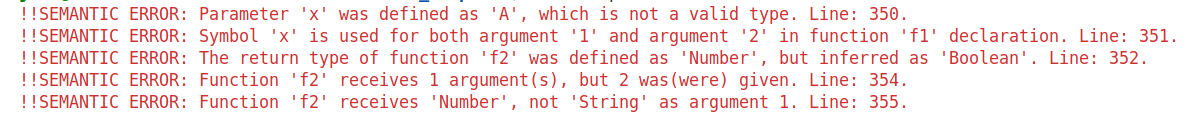
\includegraphics[width=1\textwidth]{images/func_errors.png}
\caption{Errores comunes en condicionales y ciclos}
\label{fig:errores_4}
\end{figure}

\vspace{10pt}
\section{Generación de Código}
\vspace{10pt}
\begin{thebibliography}{9}
\bibitem{aho06}
Aho, A.V., Lam, M.S., Sethi, R., Ullman, J.D.: 
Compilers: Principles, Techniques, and Tools (2nd Edition). 
Addison-Wesley (2006)

\bibitem{appel98}
Appel, A.W.: Modern Compiler Implementation in C. 
Cambridge University Press (1998)

\bibitem{llvm}
Lattner, C., Adve, V.: 
LLVM: A Compilation Framework for Lifelong Program Analysis \& Transformation. 
CGO 2004, LNCS 3161, Springer (2004)
\end{thebibliography}
\end{document}